\documentclass[11pt]{article}
\usepackage{geometry}                
\geometry{letterpaper}                   

\usepackage{graphicx}
\usepackage{amssymb}
\usepackage{epstopdf}
%\usepackage{natbib}
\usepackage{amssymb, amsmath}
\usepackage{hyperref}
\DeclareGraphicsRule{.tif}{png}{.png}{`convert #1 `dirname #1`/`basename #1 .tif`.png}

%\title{Title}
%\author{Name 1, Name 2}
%\date{date} 

\begin{document}



\thispagestyle{empty}

\begin{center}
\includegraphics[width=5cm]{ETHlogo.eps}

\bigskip


\bigskip


\bigskip


\LARGE{ 	Lecture with Computer Exercises:\\ }
\LARGE{ Modelling and Simulating Social Systems with MATLAB\\}

\bigskip

\bigskip

\small{Project Report}\\

\bigskip

\bigskip

\bigskip

\bigskip


\begin{tabular}{|c|}
\hline
\\
\textbf{\LARGE{Evacuation Bottleneck}}\\
\textbf{\LARGE{A look onto the evacuation of a cruise ship}}\\
\\
\hline
\end{tabular}
\bigskip

\bigskip

\bigskip

\LARGE{Benedek Vartok \& Johannes Weinbuch}



\bigskip

\bigskip

\bigskip

\bigskip

\bigskip

\bigskip

\bigskip

\bigskip

Zurich\\
December 2009\\

\end{center}



\newpage

%%%%%%%%%%%%%%%%%%%%%%%%%%%%%%%%%%%%%%%%%%%%%%%%%

\newpage
\section*{Agreement for free-download}
\bigskip


\bigskip


\large We hereby agree to make our source code for this project freely
available for download from the web pages of the SOMS chair. Furthermore, we
assure that all source code is written by ourselves and is not violating any
copyright restrictions.

\begin{center}

\bigskip


\bigskip


\begin{tabular}{@{}p{3.3cm}@{}p{6cm}@{}@{}p{6cm}@{}}
\begin{minipage}{3cm}

\end{minipage}
&
\begin{minipage}{6cm}
\vspace{2mm} \large Johannes Weinbuch

 \vspace{\baselineskip}

\end{minipage}
&
\begin{minipage}{6cm}

\large Benedek Vartok

\end{minipage}
\end{tabular}


\end{center}
\newpage

%%%%%%%%%%%%%%%%%%%%%%%%%%%%%%%%%%%%%%%



% IMPORTANT
% you MUST include the ETH declaration of originality here; it is available for
% download on the course website or at
% http://www.ethz.ch/faculty/exams/plagiarism/index_EN; it can be printed as
% pdf and should be filled out in handwriting
\begin{center}
		
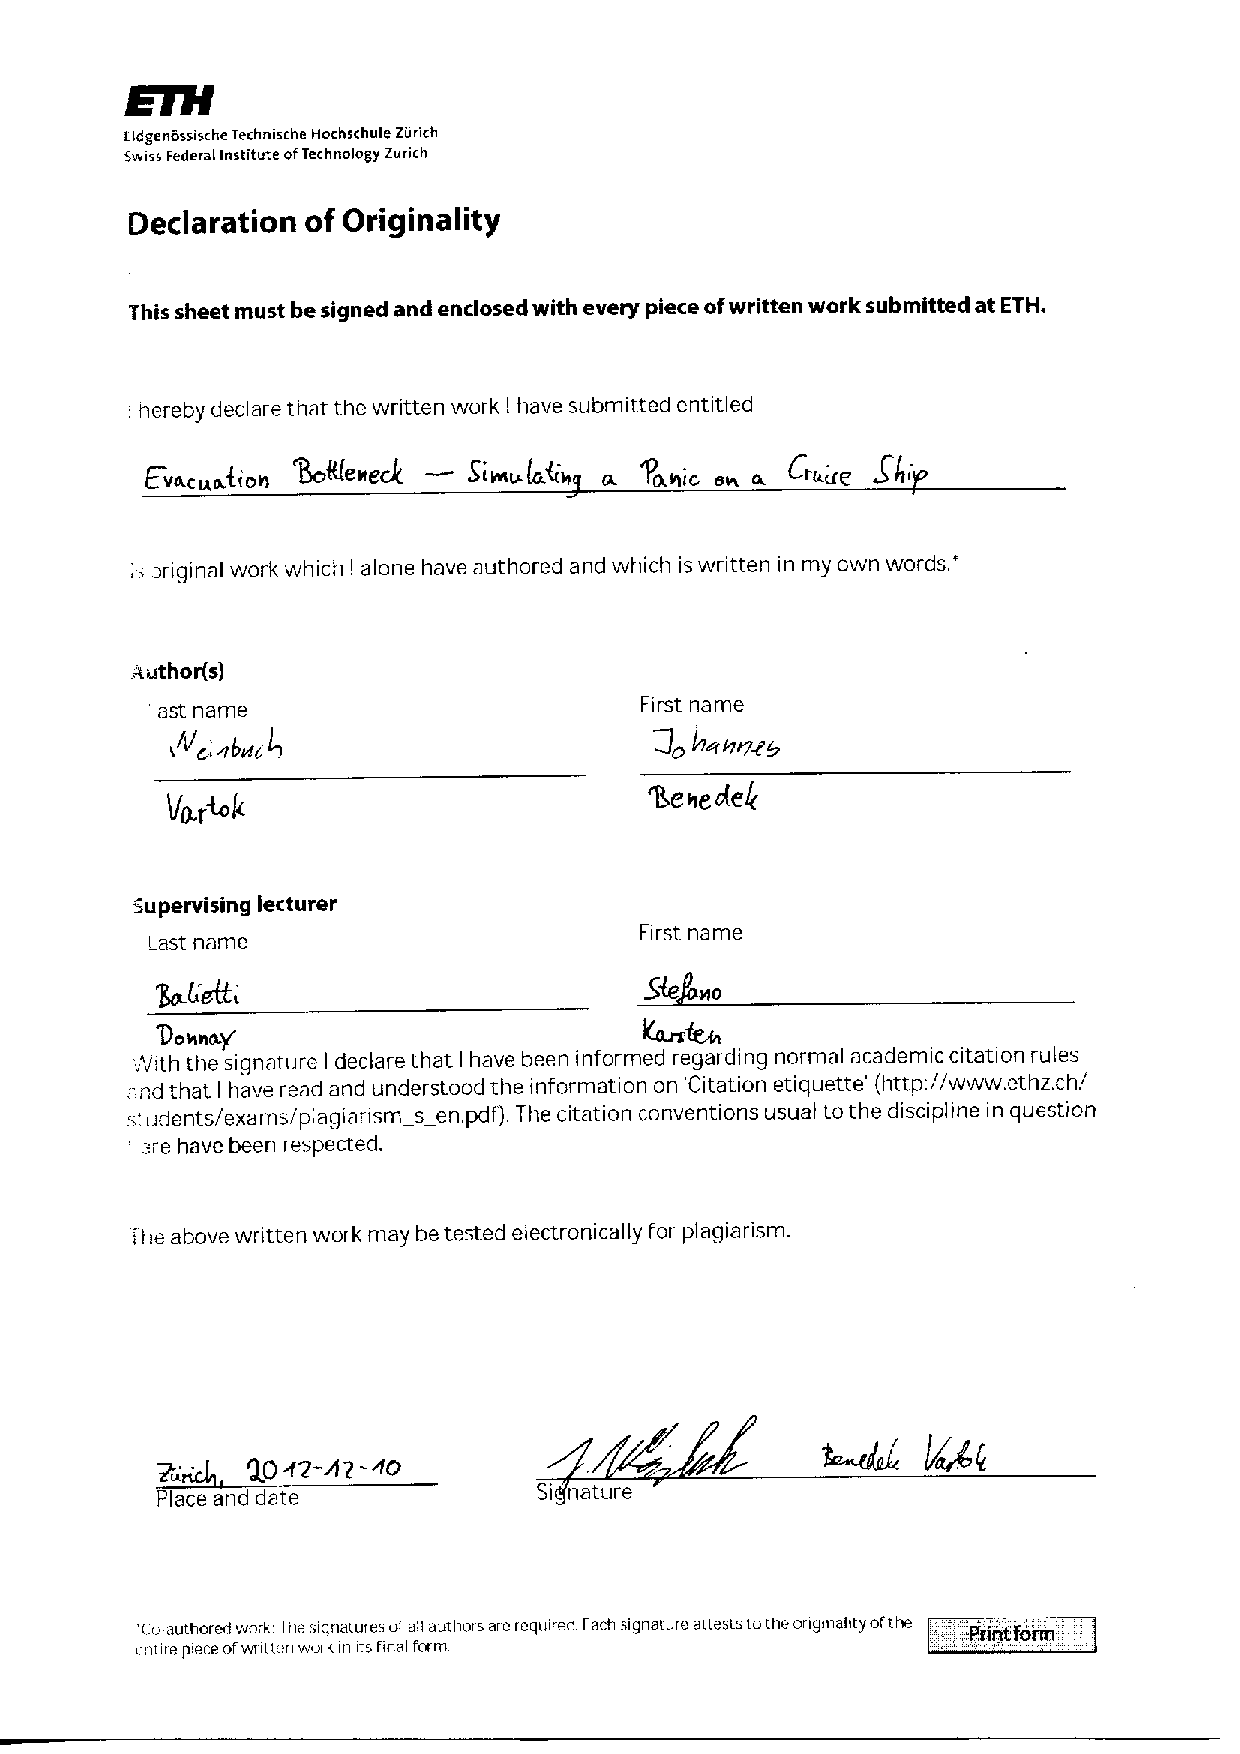
\includegraphics[scale=0.7]{images/declaration.pdf}

\end{center}
\newpage


%%%%%%%%%% Table of content %%%%%%%%%%%%%%%%%

\tableofcontents

\newpage

%%%%%%%%%%%%%%%%%%%%%%%%%%%%%%%%%%%%%%%



\section{Abstract}

This work takes a look into the evacuation mechanisms of a cruise ship in case
of an emergency.  A simple model is implemented which is used to simulate the
dynamics of such a system.  The main emphasis was on the limited capacity of
the exits, since that is the key element for a rescue boat. 


\section{Individual Contributions}

The work on this project was split among us to fit our strengths the best way
possible.  Because of his knowledge in image editing and formats, Johannes
Weinbuch focused on the image manipulation for the input and implemented the
loading of the image into MATLAB, improving the existing solutions from the
previous courses. He further took a large part of the writing for the report
and executing the simulations, which were written by Benedek Vartok.  He
evaluated which code from previous semesters could and should be reused, and
implemented the missing parts for our special case.  Also, he wrote the output
mechanisms for the simulation, so that the data could be used for analysis.


\section{Introduction and Motivations}

In January 2012, the Costa Concordia hit a rock and ran aground\cite{bbcnews}.
This event got great media attention for a long time so we decided to take a
closer look at the evacuation of a cruise ship.  The question is, what is the
best stratgy to leave the ship?  This question should for sure be answered with
one of the emergency drills, but it is always good to have some background
knowledge.

So, our key questions are: Which is the best strategy for evacuation concerning
the choice of the way towards the rescue boats. Should all passengers
dirstribute equally over the entries, or is there a better one? Also, which one
takes longer: a high panic level on a nearly empty ship or a low panic level on
a very full ship. What happens, if a boat suddenly is inoperable? How can the
reaction be optimized?


\section{Description of the Model}

The model is a big simplification of real life, otherwise it would be way too
complex to simulate.  It assumes that the ship is intact, that there is calm
sea and that the passengers are obliged to leave the ship.  A possible
explanation for this could be a machine defect which leaks explosive gas in a
badly ventilated room in the ship.  Further, we assume that the rescue boats are
like doors, which close after a certain amount of people going through them. 

Since we also assume that the other doors, for example between the rooms or
floors, are constantly open and working, we only simulate one deck, the one
with the exits to the rescue boats.  The evacuation of multiple floors in a
static building has already been researched in \cite{multilevel}. 

After these simplifications, the task left to simulate was the evacuation of a
single floor with some elements that can change.  For this task, we chose a
simple agent based modeling solution as described in \cite{helbing}.  A
passenger is treated as a particle.  It has a mass, and there are physical and
social forces, accelerating that mass so that it cannot always follow its
desired direction.  The desired direction is implemented as the shortest path
to the nearest exit.  For the exact formulae for the forces see
section~\ref{sub:movement}.

The floor is given by a deck plan for the Costa Voyager \cite{costa}. Since
these deck plans usually are made for advertisment purposes, it is to be
expected that they are not absolutely accurate.  So during image processing for
simplification of this plan, a few further assumptions were made, mainly about
the actual sizes and capacities.  We won't list them all here, because they are
also in the configuration files. 

The last element of additional complexity was added to get an idea of how the
closing of an exit works.  A switch was added to decide whether every agent
should know instantanously about the closed exit or if the knowledge spreads
over time.  The technical aspect of this is further explained in
section~\ref{sub:exitremove}.

\section{Implementation}

\subsection{Input}

\label{sub:input}

Since we had some good projects which covered similar
problems as ours, we could get some ideas from them, but at the same time
improve them.  Namely, there are \cite{multilevel} and \cite{airplane}.  As far
as the input for the simulation is concerned, we see two approaches in these
works for getting the map data into the simulation.  In \cite{multilevel}, a
simple PNG image is used to get a map into the simulation. The problem here is
that only a certain RGB color value can be read out of the image.  This can
lead to problems if the image is processed with automatic or semiautomatic
image manipulation programs, since only a minor difference in color can prevent
the generation of the desired data.  In \cite{airplane}, the image format is
even more simple.  There is only a bitmap image read into MATLAB.  Since the
bitmap images can use a colormap, MATLAB doesn't use 3 channels but a unique
number for each color in an image matrix to give every pixel its color.  This
has the same problem as the PNG solution regarding how exactly the colors have
to be set, but the different parts of the image can be separated with less
code.

We took the best of both solutions. We used the PNG-format with indexed colors.
So we have the most flexibility with very little usage of disk space.  There is
no special ``wall color'' or anything like that, just a simple rule how the
colormap is read: Color 0 of the map specifies walls, color 1 free space.
Then, there can be any number of spawn zones.  Spawn zones are the areas in the
image, where new agents can be placed. With different spawn zones, it is
possible to account for different situations: A ballroom is different from a
staircase.  The number of spawn zones is specified in the configuration file.
At last, there is an arbitrary number of exits.  Again, each exit can have its
own parameters or can even be handled specially in the program's code. 

\begin{figure}[h]
	\centering
	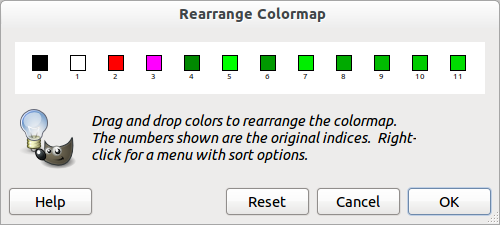
\includegraphics[scale=0.5]{images/gimp.png}
	\caption{Screenshot of the Rearrange Colormap dialog in Gimp 2.6.11}
	\label{gimpscreenshot}
	
\end{figure}
To manipulate the colormap, any slightly sophisticated image manipulation
program should suffice. We used the free software Gimp \cite{gimp}. It has a
very convenient command which allows the user to rearrange the colormap. This
is shown in figure~\ref{gimpscreenshot}.

\subsection{The Simulation Routines}
\label{sub:The simulation Routines}

\subsubsection{Code Reuse from Multilevel Evacuation}

Since this project has very similar foundations as \cite{multilevel} (like the
forces used in the model), we were able to use a lot of code and some design
decisions from their program.  Some of the structure needed to be changed to
implement our custom features, but for example the utility functions for the
Fast Sweeping algorithm (\texttt{fastSweeping.c}), generating gradients
(\texttt{getNormalizedGradient.c}) and the linear interpolation
(\texttt{lerp2.c}) which the other group wrote in C were copied without
modification into our code-tree.

\subsubsection{General Structure}

\label{sub:structure}

During the entire program run, one single big structure is used to hold and
pass around the state of the simulation.

At first, this structure is initialized with the fields that are given in the
configuration file by \texttt{loadConfig}\footnote{The MATLAB implementation of
our functions is in the \texttt{code} directory: \texttt{loadConfig} can be
found in the file \texttt{code/loadConfig.m} etc.}.  Then, \texttt{initialize}
runs over the struct and calculates some data needed in the simulation, such as
the vector fields needed for the wall and exit force fields using the
\texttt{fastSweeping} method which we got from \cite{multilevel}.

\subsubsection{Main Loop}

\texttt{simulate} is the routine we call when we do an entire simulation.  It
uses the \texttt{loadConfig} and \texttt{initialize} functions to initialize
its runtime data, then it does the loop calculating forces, adding new agents,
progressing the agents, updating the exit vector fields, potentially plotting
and saving frames and collecting data.

These steps will be explained in detail in the following sections.

\subsubsection{Agent Placement}

As mentioned in section~\ref{sub:input}, our model of the ship has different
spawning zones where new agents can start out at.  The way we implemented it,
in every step of the simulation loop it is checked whether there are any
remaining agents that need to be placed (i.e. agents which are not in the
simulation yet).  If there are, then for every agent the program chooses a
random point in the spawning zones and places him there, unless it detects that
the agent would collide either with walls or other agents.  In that case, the
routine tries the placement for that agent up to five times, each time with a
new random position.  If the agent couldn't be placed, then he will have a
chance to spawn in the next time step.

This method was implemented in \texttt{placeAgents}.  In the same method, the
basic properties of the agent get assigned, like the starting zero velocity and
a random radius.

\subsubsection{Agent Dynamics}
\label{sub:movement}

To simulate the movement of the agents in this physical model, different forces
need to be calculated in every step on every agent.  All of the force formulae
have been taken from \cite{helbing}.  These forces have been separated into the
following functions which are called by \texttt{simulate}:

\begin{description}

\item[\texttt{addDesiredForces}] is responsible for making the agents seek the
exits of the layout, in our case the rescue boats.

This is accomplished by giving an agent a ``desired'' velocity vector pointing
along the shortest path to the nearest exit.  The vector is sampled and
interpolated (using \texttt{lerp2} from \cite{multilevel}) from a vector field
which is calculated at the beginning (see \ref{sub:structure}) of the
simulation and when the exits change (see \ref{sub:exitremove}).

Using this desired vector $\vec{e}$ we can say what force addition the agent gets:

\[ \vec{F}_\text{desired} = m \frac{v_0 \vec{e} - \vec{v}}{\tau} \]

where $m$ is the agent's mass, $v_0$ is his target speed, $\vec{v}$ is
his current velocity vector and $\tau$ is a characteristic time determining how
fast the desired velocity should be reached.

\item[\texttt{addInterAgentForces}] models the repulsive forces between agents:
They do not want to get too close together and if they touch, they have to be
kept apart physically and some friction appears.  The model we use has this
formula:

\[ \vec{F}_\text{agents} = \big(A e^{(r-d)/B} + k \max\{0, r-d\}\big) \vec{n} +
                     \kappa \max\{0, r-d\} \Delta \vec{v} \cdot \vec{t} \]

where $r$ is the sum of radii of both agents, $d$ is the distance between the
center points of the agents, $\vec{n}$ is the normalized vector between the two
agents, $\vec{t}$ is the tangential vector and $\Delta \vec{v}$ is the velocity
difference vector.  $A$ influences the magnitude of the ``social'' repulsive
force, $B$ specifies a factor for the range of influence for this force, $k$
gives the strength of the physical separation force and $\kappa$ is a friction
coefficient.

For finding possible agent pairs to calculate the function on we used the naive
approach of checking every possible pairing with two nested loops and then
using a cutoff distance to avoid calculating this complicated force expression
when it's too small to matter anyways.  This method has complexity
$O(N_\text{agents}^2)$ which is far for optimal; we also tested the Range Tree
implementation of \cite{multilevel} for our program, however benchmarks didn't
show a noticeable gain in efficiency.

\item[\texttt{addWallForces}] calculates agents avoiding and experiencing
resistance from walls.  Just like agent-agent repulsion, this force has a
``social'', a physical and a frictional component:

\[ \vec{F}_\text{walls} = \big(A e^{(r-d)/B} + k \max\{0, r-d\}\big) \vec{n} -
                    \kappa \max\{0, r-d\} (\vec{v} \cdot \vec{t}) \vec{t} \]

where $r$ is the radius of the agent, $d$ is his distance from the wall,
$\vec{n}$ is the wall normal vector, $\vec{t}$ is the wall tangent vector and
$\vec{v}$ is the agent's velocity vector.  The coefficients are the same as in
$F_\text{agents}$.

Accessing the wall distances and normals is done similarly to
\texttt{addDesiredForces}, with precalculated fields using the Fast Sweeping
method.

\item[\texttt{progressAgents}] applies the forces from the above listed
functions, using them to update the agents' positions and velocities for the
next simulation step.

To accomplish this, the leap-frog integration scheme was used.  In every step,
the following recalculations of the velocities and positions of the agents take
place:

\begin{align*}
\vec{v} &= \vec{v} + \Delta t \cdot \frac{\vec{F}}{m}  \\
\vec{x} &= \vec{x} + \Delta t \cdot \vec{v}
\end{align*}

This method is fairly well suited for physical simulations with forces such as
these.  However, extra measures were taken to improve the stability of our
program:  Before doing any further calculations with them, the velocities and
forces get clipped to a configurable maximum magnitude to avoid instabilities
for too high step-sizes or too strong force parameters.

Without this, the simulation of some agents might get out of control if they
get too close to walls or to other agents and behave in unphysical ways.

This function also checks whether some agents have entered a non-full exit zone
(a rescue boat) and if the exit got full from them, it closes that one.  What
exactly happens then is explained in the next section.

\end{description}

\subsubsection{Removing Filled Exits}
\label{sub:exitremove}

In our model we have several exit zones, each with a maximum capacity (since
they are rescue boats with limited size).  Because of that the simulation needs
to take it into account when one of them gets filled: It needs to remove the
exit and update the vector fields for the desired velocities which the agents
use to find the nearest exit.  For this update we modeled and implemented two
different approaches which can be chosen in the configuration file.

The first one simply recalculates the entire vector field when an exit is
closed with the Fast Sweeping method, just like in the initilization, but with
the full exits removed.  The update is instantaneous, so every agent on the
entire ship reacts to it immediately.  This is somewhat unrealistic, which is
why we came up with the second method.

Instead of updating the entire vector field right away, we can just calculate
the updated field and use that to update growing regions.  To be exact, when an
exit closes, a circle starts growing around at a configurable rate, and in this
area the new destination vector field is used.  That way, at first only agents
close to that exit react to the change, then over time the more distant agents
also ``notice'' the filled exit and go for a different one.

The circle-shaped destination field update is implemented in
\texttt{progressDestFields}.

\subsection{Output and Plotting}
\label{sub:output}

Our program has two plotting functions:

\texttt{plotFloor} draws the ship's layout and all the agents on it in the
current simulation state.  It is called from \texttt{simulate} in every loop
iteration and the resulting picture is saved to \texttt{code/frames/}, but only
if the option for saving frames has been enabled in the configuration file.

\texttt{plotExitedAgents} is called at the end of the simulation and creates
time series plots of the rescue boat occupations.

Also the program saves its entire state data object to a file in
\texttt{code/frames/} at the end, which includes other information as well,
such as the time needed for all agents to reach the exits and the time series
of the total escaped agents.

\section{Simulation Results and Discussion}

\subsection{Passenger distribution} % (fold)

If we plot the exited agents over a time axis for each exit, we can see that
the boats tend to be filled in a sequential way (See Figure~\ref{distribution11} and~\ref{distribution33}).
This means, a new boat mostly
gets frequented if the old boat is already full.  This effect is very strong
and good to see if we have only few passengers, but also if there are many, a
tendency towards this can be observed. The only thing, that interferes with this 
observation is, that at the beginning, two boats are filled at the same time.
This is because some agents are placed so that they have a shorter distance to the left.

\begin{figure}[h]
	\centering
	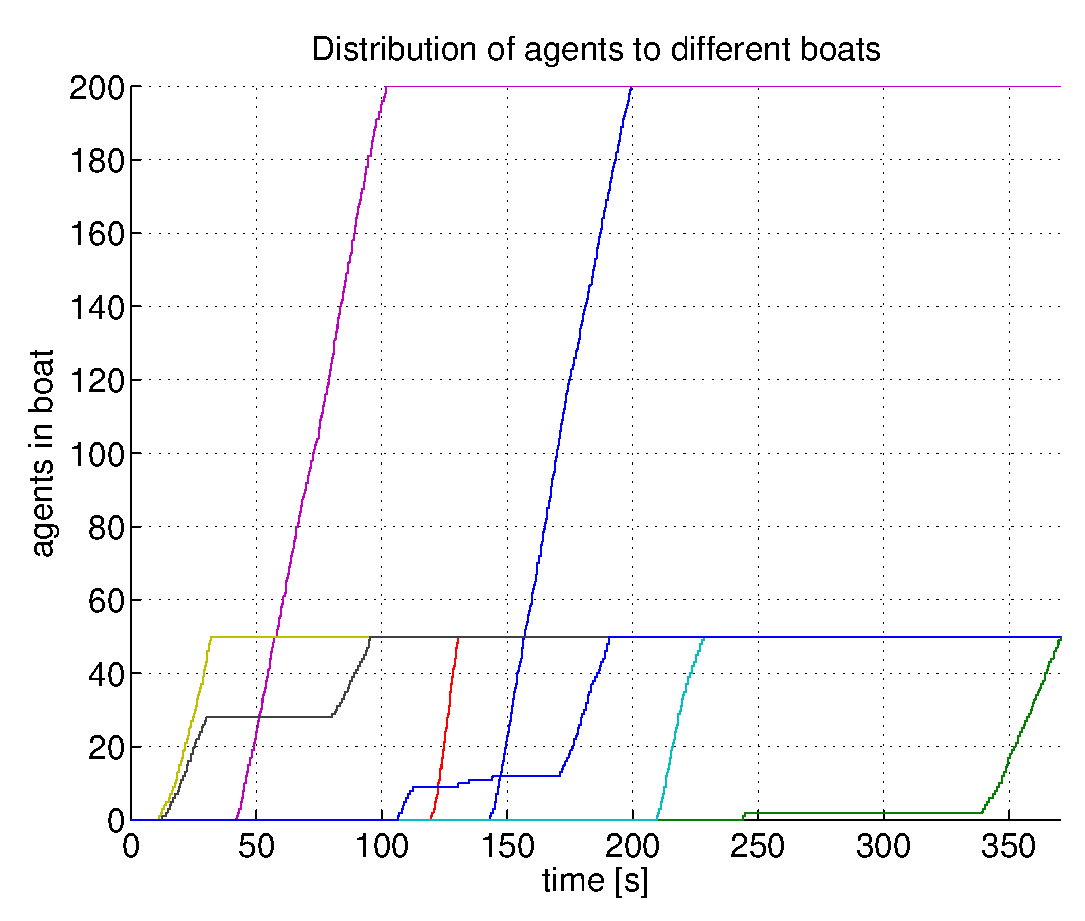
\includegraphics[scale=0.5]{images/distribution11.eps}
	\caption{Plot of the filling of the rescue Boats on a ship with 700 Agents, \(v_0=1.5\frac{m}{s}\).
	Each line represents a different rescue boat.}
	\label{distribution11}
\end{figure}

\begin{figure}[h]
	\centering
	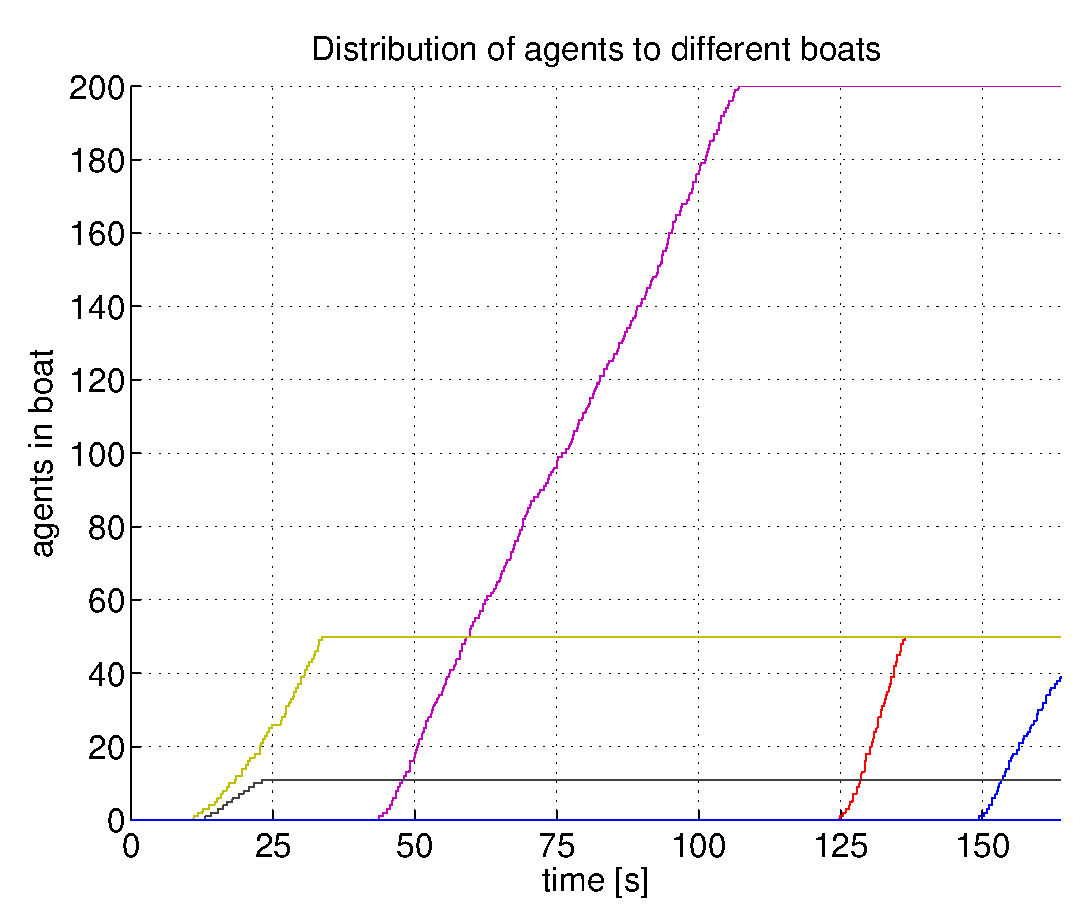
\includegraphics[scale=0.5]{images/distribution33.eps}
	\caption{Plot of the filling of the rescue Boats on a ship with 350 Agents, \(v_0=1.5\frac{m}{s}\).
	Each line represents a different rescue boat.}
	\label{distribution33}
\end{figure}

Although there could be numerous
reasons for this to happen, in reality a more distributed and parallel filling
of the boats is expected.  The simulation is based on a model which takes the
distance to the nearest exit as the indicator for the desired direction.  In
reality, people want to get out of the ship the fastest way possible,
especially if there are only limited capacities on the boats.  This suggests
that the nearest exit is not the best strategy to get out fast.  On the
specific geometry of the Costa Concordia, the corridor from bow to stern ends
more on the starboard (right) side.  The agents follow the shortest path and
start to jam up, while on the left there are no obstacles.
Without regard to the beginning, two boats get used in parallel only if there are many agents.
This can be explained by the jam, so people get pushed back towards the other 
boat. Also, if a boat is empty, the Crowd can seperate into two parts: One,
that is nearer to the next boat on the same side and one, which was further
away from the empty boat, which now has the nearest boat on the other side.

The expectation for reality is that people would recognize that the nearest 
boats take more time to reach than the ones further away. Thus, they would 
distribute more equally over the different boats.




% subsection Passenger distribution (end)

\subsection{Panic Level} % (fold)
As described in \cite{helbing}, a bigger desired velocity \(v_0\) 
can lead to longer times in evacuation.
At a higher panic level, people want to go faster, but it can ake longer to get out.
When \(v_0\) is below 1.5m/s, we could reproduce the results of decreasing evacuation times
both with many and few agents, as seen on Figures \ref{evactimes1to11} and \ref{evactimes23to33}.

\begin{figure}[h]
	\centering
	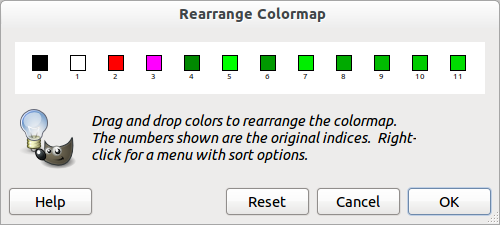
\includegraphics[scale=0.5]{images/gimp.png}
	\caption{Platzhalter}
	\label{evactimes1to11}
	
\end{figure}

\begin{figure}[h]
	\centering
	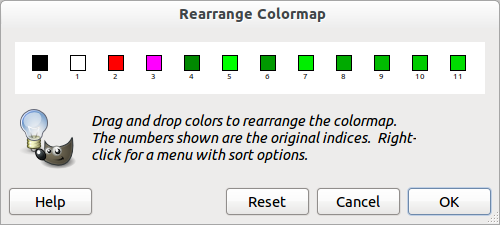
\includegraphics[scale=0.5]{images/gimp.png}
	\caption{Platzhalter}
	\label{evactimes23to33}
	
\end{figure}

However, with higher values for \(v_0\), we could not reproduce the results, because
agents got pushed into walls and remained stuck there. In Figure~\ref{evactimes1to11},
we had two agents stuck in Walls at \(v_0 = 1.4m/s\), so we looked at the results,
and set the finish time to the value, when the last agent before them left
the ship. This introduces an error, which only gets bigger with higher values of \(v_0\).

To circumvent this, a simulation with a smaller timestep was run, but even with the timestep 
being a millisecond, we still got agents stuck in walls. An example is shown in Figure~\ref{stuckinwall}. This is a part during the simulation with \(v_0 = 3.8m/s\) and a timestep of a millisecond.

A timestep of a millisecond means, that an agent, moving at five meters per second,
goes a distance of 5 millimeters per timestep. Since the agents get pushed into walls
at these rather precise steps of movement, an even smaller timestep will likely yield similar results. 

\begin{figure}[h]
	\centering
	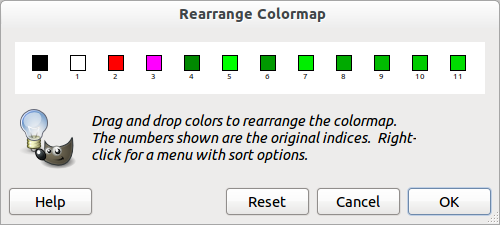
\includegraphics[scale=0.5]{images/gimp.png}
	\caption{Platzhalter}
	\label{stuckinwall}
	
\end{figure}

Since we cannot answer our question, wether a high panic level (which means a high value for \(v_0\))
with few people
or a low panic level with many people is faster, we try to find reasons for this outcome.

A timestep too big can be excluded from the reasons, as we have seen before.
We chose the parameters to be the same as in \cite{helbing} on page 488.
They have been found suitable to simulate people leaving a room.
The difference to our case is, that we have more walls nearby and
because of that, we get a situation where more pressure is applied from more sides. 
Since that is a remarkable difference to the situation of a single room with one door, 
it is plausible, that the parameters are not suited for high densities of people in 
narrow places. 

Of course, this could also be interpreted as people being hurt, but since
we did not take this into account for our model, no relevant statements can
be made. It should be part of a next simulation to account for the sum of 
physical forces acting upon an agent. If they are too big, the agent gets hurt.
In our case, this would be a realistic assumption, since a ship with limited
exit possibilities can make the people feel trapped rather fast and is so more
likely to trigger panics than other places.



% subsection Panic Level (end)
\subsection{Closed Exits} % (fold)
\label{sub:Closed exits}

In the simulation, two ways were defined to react to a full boat.  First, there
was an instantanous update on the whole ship.  This is a model for an
announcement over speakers over the whole ship.  The agents adapt their
direction immediately, which can be seen on a video of the simulation.  This
behaviour is realistic in a case when there are not too many people who aren't
panicking.

The second way is that the information is spread in a circle around the exit.
This shall model a simple communication between agents that takes time.  With
this simple rule of updating the directions, the behaviour is much more
realistic, even though the rule doesn't account for the number of people
nearby.  This means that the information spreads, even if there is nobody.
However, an interesting phenomenon during the updates can be observed:  While
the people near the exit try to get to the next one, they get pushed back by
the others who don't know of the change yet.

The flaw of this is that a slow expansion rate leads to more pushing, but if
it's too slow, even an agent that escaped can be run against the border of the
expansion circle.  This is then seen as the agent stopping, even if there is
nothing blocking his path. That happens because the agent is faster than the
expansion rate of the information. From observations in the simulation, we
found \(0.5\frac{m}{s}\) to look mostly like we expected it, even though
occasionally there are still some agents slowed down by the expansion rate.

The effect of the pushback on the evacuation time is very small, because of
numerous bottlenecks before the actual exit.

TODO: PLOT EINFÜGEN

% subsection Closed exits (end)

\section{Summary and Outlook}

\section{References}
\bibliographystyle{plainnat}


\begingroup 
\renewcommand{\section}[2]{}%
\begin{thebibliography}{9}

	\bibitem{bbcnews}
		\url{http://www.bbc.co.uk/news/world-europe-16563562}, 9.12.2012

	\bibitem{multilevel}
	\emph{Modelling Situations of Evacuation
in a Multi-level Building} , 
Hans Hardmeier, Andrin Jenal, Beat Küng, Felix Thaler, Zurich, April 2012

	\bibitem{helbing}
		\emph{Simulating dynamical features of escape panic},
		Dirk Helbing, Ill\'es Farkas, Tam\'as Vicsek, Nature, 28. September 2000

	\bibitem{costa}
		\url{http://www.kreuzfahrtberater.de/deckplan.php?schiff=Costa+Voyager&bf&dpe=2}

	\bibitem{airplane}
		\emph{Pedestrian Dynamics Airplane Evacuation Simulation},
		Philipp Heer, Lukas Bühler, Zurich, May 2011
	\bibitem{gimp}
		\url{http://www.gimp.org/}, 9.12.2012
\end{thebibliography}
\endgroup



\end{document}  



 
